% !TEX root = omar-thesis-proposal.tex
\vspace{-25pt}
\section{Introduction}\label{motivation}
% \begin{quote}\textit{The recent development of programming languages suggests that the simul\-taneous achievement of simplicity 
% and generality in language design is a serious unsolved 
% problem.} -- John Reynolds, 1970 \cite{Reynolds70}\end{quote}
%%One might exp ``generality''
Well-designed general-purpose programming languages are remarkably stable: they rarely need to be revised or forked into dialects, because programmers can express the constructs that they need just as well in orthogonal libraries. %Instead, . . %Indeed, a preponderence of new dialects is clear evidence against claims of generality.  %Not all useful abstractions can be  realized, when considered comprehensively, as libraries.% The problem of achieving both simplicity and generality simultaneously with a single system remains unsolved. 
Abstraction mechanisms informed by type theory, like  the ML module system \cite{MacQueen:1984:MSM:800055.802036}, have put this ideal within reach. 
Yet despite their expressive power, new {dialects} of languages like ML continue to arise. Why is this?

% Unlike libraries organized by a module system, language dialects are not trivially composable.%Constructing a software system using libraries written in different dialects is difficult because they cannot always be composed. %This suggests that library-based mechanisms are still not general enough to encompass many desirable modes of expression.   %Library implementations are not yet satisfying.
%Why would a well-informed programmer consider forming a new dialect? 
Perhaps the most common justification is that the \emph{syntactic cost} of a desirable construct is not  preserved when it is expressed using general-purpose mechanisms. %Syntactic cost is often assessed qualitatively \cite{green1996usability} (though quantitative metrics can also be defined). 
For example, the semantics of regular expressions can be expressed using abstract data types (which in ML are a mode of use of the module system), but as we will detail in Sec. \ref{sec:syntax}, this presents some syntactic difficulties. For programmers in problem domains  where regular expressions are common, e.g. bioinformatics, it is tempting to design a ``domain-specific'' dialect that differs only in that it includes derived syntax (i.e. ``syntactic sugar'') for regular expression patterns. There is no shortage of tools that aid in the construction of such syntactic dialects (e.g. Camlp4 \cite{ocaml-manual}, SugarJ \cite{erdweg2011sugarj}, SugarHaskell \cite{erdweg2012layout} and many others).%Put another way, such embeddings may not preserve the cognitive cost associated with a construct (qualitative criteria are generally used to establish this \cite{green1996usability}). 

Somewhat more rarely, dialects are motivated by the need to extend a general-purpose language with new derived semantic constructs, i.e. constructs that cannot be expressed as purely syntactic sugar, but where the general-purpose language is a suitable translation target. As a minimal example, consider System \textbf{F}, i.e. the polymorphic lambda calculus (perhaps the simplest general-purpose language) \cite{pfpl}. If we wanted to express record types in \textbf{F}, we could not do so simply with derived syntax. We could, however, develop a dialect that included the type and term operators relevant to records, specifying their static semantics directly but their dynamic semantics by translation to the polymorphic lambda calculus (using a standard Church-style encoding).\todo{couple more sentences} %Constructs specified by a type-directed translation like this can be considered \emph{derived semantic constructs}.


% express record types as syntactic sugar over the simply-typed lambda calculus with  binary product types.\footnote{Pairs can of course be expressed as syntactic sugar atop records, though one could argue that using binary products as the more primitive concept is simpler.} The static semantics need to be extended with new type and term operators. However, the simplest way to express the dynamic semantics of the newly introduced term operators is by translation to nested binary products, so we can leave the operational semantics alone. \todo{fill this out} %For example, there are dozens of constructs that go by the name of ``records'' in various languages, each defined by a slightly different collection of primitive operations. \todo{examples} %, encouraged  historically  by the availability of tools like compiler generators and,  more recently, language workbenches \cite{workbenches} and DSL frameworks \cite{dsl}. Unfortunately, taking this approach makes it substantially more difficult for clients to import high-level abstractions orthogonally. 

The problem with designing new language dialects in these situations is that a program written in one dialect cannot safely and idiomatically interface with libraries written in a different dialect. %At best, one can hope that the compilers for the two languages target a common intermediate language,  
To do so would require combining the two dialects into a single language, but there is no systematic method to do so, much less one that guarantees that important metatheoretic properties established about each dialect in isolation will be conserved. As a simple example, two dialects might be known to have an unambiguous concrete syntax in isolation, but if the syntax is na\"ively combined, ambiguities could easily arise. %the ideas housed in one dialect are often only available to programmers willing to do without ideas housed in other dialects. 
%It is thus infeasible to simply allow different contributors to a software system to choose their own favorite dialect for each component they are responsible for. %A complex software system written in multiple distinct language dialects is far too unwieldy for it to be viable. 
Without strong modular reasoning principles to rely upon, it is difficult to construct large software systems and ecosystems. 
%This means that it is difficult to construct large software systems and ecosystems from components written in different dialects. 
The only reasonable approach for software engineers who must program ``in the large'' is to eschew constructs housed in dialects and settle on a single common language, where they can  rely on the guarantees provided by its type and module system. %The designers of these languages may slowly adopt the most generally useful new ideas. 
This has left many useful constructs for programming ``in the small'' obscure.% It is safe to say that in contemporary times, language dialects should be considered harmful. % It is little wonder that many programmers eschew esoteric language dialects in favor of languages that stopped evolving decades ago.

\section{Contributions}
Our aim in this thesis is to make dialect formation less frequently necessary by designing language mechanisms that give library providers the ability to express derived syntactic and semantic constructs from within the language, in a manner that ensures that these constructs can be reasoned about separately and composed arbitrarily. 

%Such mechanisms are colloquially known as \emph{extension mechanisms} because the sorts of constructs they are used to express are those that would otherwise require extensions to the language itself. %Defining a new construct then corresponds to the usual notion of language extension. We will make this intuition more precise later.


%in languages without such mechanisms, expressing such constructs would require extensions to the language itself (a better qualifier might thus be \emph{extension-mitigating}). %We will make these notions more precise as we continue. %Thus, these mechanisms precisely capture the notions of language extension and language composition.



%The mechanisms we propose are designed to decrease the number of constructs that need to be built in \emph{a priori} by a language designer. However, there are still some basic syntactic and semantic decisions that must unavoidably be made. 

To provide a coherent vehicle for these mechanisms, we will introduce a new general-purpose language called Wyvern. Let us briefly summarize its organization. Syntactically, Wyvern has a layout-sensitive textual concrete syntax (i.e. indentation is meaningful). This choice is not fundamental to our proposed mechanisms, but it will be useful for a class of examples that we will discuss later.  Semantically, Wyvern consists of a \emph{module language} and a \emph{core language}. The module language is based directly on the Standard ML module language, with which we assume familiarity for the purposes of this proposal \cite{harper1997programming}. The core language (i.e. the language of types and expressions) is split into an \emph{external language} (EL) and an \emph{internal language} (IL). The semantics of EL constructs are specified by a type-directed translation to the much simpler IL. Notionally, this can be thought of as simply a shifting of the first stage of a type-directed compiler into the language specification \cite{tarditi+:til-OLD}. The internal language we will use is the polymorphic lambda calculus with binary product and sum types and recursive types (features like state and exceptions could also be included, but for simplicity, we will omit them) \cite{pfpl}. %Again, we will make these statements more precise as we continue.%The external language provides local type inference \cite{Pierce:2000:LTI:345099.345100}. % (for the purposes of this work).

We will begin by describing Wyvern's mechanisms for expressing new forms of derived concrete syntax, assuming for the moment that the EL is otherwise specified in a standard way, in Section \ref{sec:syntax}. We then turn in Section \ref{sec:semantics} to a mechanism for introducing new semantic constructs -- in particular, new base types and operators -- into the EL. Constructs that are built in to languages like ML, like $n$-ary tuples/records, labeled sums and others, can in Wyvern be realized as modes of use of this mechanism. In both cases, the mechanisms can be broadly understood as novel forms of \emph{static metaprogramming}. Users define each new syntactic and semantic construct by writing code that generates terms and types. This code is  evaluated statically, in the course of typechecking EL terms.


%Languages that are organized around mechanisms like these are colloquially known as \emph{extensible languages}. 


For each mechanism that we introduce, we will first demonstrate its expressive power by showing how constructs that are, or would need to be, built directly in to contemporary languages can in Wyvern be expressed in libraries. To demonstrate that these mechanisms are theoretically sound, we will then develop a formal specification and proofs of various important metatheoretic properties. The most interesting of these will be various \emph{modular reasoning principles} that guarantee that user-defined syntactic and semantic constructs can be reasoned about separately and then used together in any combination. These justify our classification of Wyvern as a \emph{modularly extensible programming language}.



%Designing a modularly extensible language is a challenge because giving away too much control can easily make reasoning about program behavior difficult and lead to problems that arise only when extensions are used at the same time. For example, a library provider given free reign over syntax and semantics could introduce parsing conflicts, violate {type safety}, and  interfere with other extensions. We aim to design mechanisms that eliminate these possibilities, while providing a degree of expressive power sufficient to express a variety of constructs that are, or would need to be, built directly in to today's languages. %ll constructs that can be defined using a mechanism we will introduce can be reasoned about separately and composed arbitrarily.% With these mechanisms, we anticipate dialect formation being far less common. %Indeed, all of these problems have plagued previous  designs.



% Common dialects of ML that suffice for \cite{harper1997programming}. %We will . 

   %Our challenge will be to design mechanisms that achieve these goals while also being powerful enough to express features that today require dialects.%Our challenge will be to design such extension mechanisms, while still retaining significant expressive power -- we wish to permit library-based expression of a range of features that today are, or would need to be, built into a system by its designers.%It can also make it more difficult to define new sorts of tools for working with the language because they cannot rely on there being a fixed abstract syntax (the canonical \emph{expression problem}). For programmers, 
%It can make it difficult to understand and reason about the type of an unfamiliar term, a critical facet of program comprehension (the \emph{typing discipline problem}).

%So our goal will be to design extension mechanisms that handle these metatheoretic and composition-related issues while still  permitting library-based expression of a range of features that today are, or would need to be, built into a system by its designers. %More specifically, we will show how to delegate control, in a methodical manner, to \emph{static functions}, i.e. user-defined functions written in a \emph{static language}. By layering these mechanisms over a fixed typed internal language, constraining the static language appropriately and validating the code it is used to generate, we will retain key  metatheoretic properties and arrive at powerful modular reasoning principles. %By associating these static functions with type constructors, forming \emph{active type constructors},  we will further show how they can enjoy a usage profile essentially identical to that of built in features. % while maintaining key metatheoretic properties and modular reasoning principles. % By keeping the abstract syntax fixed and layering these mechanisms atop a fixed typed internal language (essentially lifting the first stages of compilation into the language), we avoid most aspects of the expression problem. %By delegating control to user-defined functions provided alongside user-defined type constructors (forming \emph{active type constructors}), we can give library providers substantially more control over these features of the system. 
%We structure each mechanism that we introduce as a \emph{bidirectional type system} combined with an  \emph{elaboration semantics} targeting a fixed typed internal language. 
%By constraining these functions and enforcing critical abstraction barriers between extensions, we will ensure key metatheoretic properties of the language and system components and guarantee that extensions can be reasoned about modularly. %We call user-defined types that introduce new features into the system in this way \emph{active types}.  % also highly expressive.
%But taking a \emph{language-internal approach} to implementing a feature is the most practical. If a feature can be realized by creatively using existing language constructs and distributed as a library, clients face fewer barriers to adoption because it is easy to integrate library-based features into existing projects gradually and granularly and they leverage well-understood and well-developed mechanisms.
% But taking this approach is often \emph{not} possible today %We call designs \emph{monolithic programming systems}.

%To realize a new abstraction or system behavior, such experts can consider either a \emph{language-internal approach}, where they work within an existing language and distribute their solutions as libraries, or a \emph{language-external approach}, where they create a new, distinct programming system (often centered around what has come to be called a new \emph{domain-specific language} \cite{dsl}) or extend an existing system by some mechanism that is not part of the language itself, such as an extension mechanism supported by a {particular} compiler, editor or other tool.

%The result of this work will be the design of a \emph{modularly extensible programming language} called Wyvern.   and end with a brief foray into editor services in Sec. \ref{sec:editor-services}.\todo{fix sections}

\section{Modular Derived Syntax}\label{sec:syntax}
Most contemporary computer programming languages specify a textual concrete syntax. Because it serves as the language's human-facing user interface, it is common practice to include  derived syntactic forms (colloquially, \emph{syntactic sugar}) that capture common idioms more concisely or naturally. % (i.e. considering cognitive dimensions \cite{green1996usability}). 
For example,  list syntax is built in to most dialects of ML, so that instead of having to write \lstinline{Cons(1, Cons(2, Cons(3, Nil)))}, a programmer can equivalently write \lstinline{[1, 2, 3]}. Many languages go further, building in syntax associated with other types of values, like vectors (SML), arrays (Ocaml), commands (Haskell) and syntax trees (Scala).  %The desugaring from the latter to the former is specified by the language itself. %Typically, the language designer controls what forms of derived syntax are built in to the language.

Rather than privileging  particular data structures, Wyvern instead exposes mechanisms that allow library providers to introduce new derived syntactic constructs on their own. %Lists need no special consideration from the language specification.
%The purpose of this section is to motivate and then introduce Wyvern's syntax extension mechanisms. %For forms with a clear analogy to a form in Standard ML, we will assume the  semantics are analagous without providing details.
To motivate our desire for this level of syntactic control, we begin in Sec. \ref{sec:examples} with the example of regular expression patterns expressed using abstract types, showing how the usual workaround of using strings to introduce patterns is not ideal. We then survey existing syntax extension mechanisms in Sec. \ref{sec:syntax-existing}, finding that they involve an unacceptable loss of modularity and other undesirable trade-offs. In Sec. \ref{sec:syntax-contributions}, we outline our proposed mechanisms and discuss how they resolve these issues. We conclude in Sec. \ref{sec:syntax-timeline} with a timeline for remaining work.


\subsection{Motivating Example: Regular Expression Syntax}\label{sec:examples}
Let us begin by taking the perspective of a \emph{regular expression} library provider. Recall that regular expressions are a common way to capture patterns in strings \cite{Thompson:1968:PTR:363347.363387}. We will assume that the abstract syntax of {patterns}, $p$, over strings, $s$, is specified as below:\[p ::= \textbf{empty} ~|~ \textbf{str}(s) ~|~ \textbf{seq}(p; p) ~|~ \textbf{or}(p; p) ~|~ \textbf{star}(p) ~|~ \textbf{group}(p)\]
The most direct way to express this abstract syntax is by defining a recursive sum type \cite{pfpl}. Wyvern supports these as case types, which are analagous to datatypes in ML:

\begin{lstlisting}[numbers=none]
casetype Pattern
  Empty
  Str of string
  Seq of Pattern * Pattern
  Or of Pattern * Pattern
  Star of Pattern
  Group of Pattern
\end{lstlisting}

However, there are some reasons not to expose this representation of patterns directly to clients. First, patterns are usually identified up to congruence. For example, $\textbf{seq}(\textbf{empty}, p)$ is congruent to $p$. It would be useful if congruent patterns were indistinguishable from the perspective of client code. Second, it can be useful for performance reasons to maintain additional data alongside patterns (e.g. a corresponding finite automata here) without exposing this ``implementation detail'' to clients. Indeed, there are many ways to implement regular expression patterns, each with different performance trade-offs. For these reasons, a better approach is to define the following \emph{module type} (a.k.a. \emph{signature} in SML), where the type of patterns, \lstinline{t}, is held abstract. The client of any module \lstinline{P : PATTERN} can then identify patterns as terms of type \verb|P.t|. 
Notice that it exposes an interface otherwise isomorphic to the one available using a case type:

\begin{lstlisting}[deletekeywords={case},numbers=none]
module type PATTERN
  type t
  val Empty : t
  val Str : string -> t
  val Seq : t * t -> t
  val Or : t * t -> t
  val Star : t -> t
  val Group : t -> t
  val case : (
    'a -> 
    (string -> 'a) ->
    (t * t -> 'a) ->
    (t * t -> 'a) ->
    (t -> 'a) ->
    (t -> 'a) -> 
    'a)
\end{lstlisting}

\paragraph{Concrete Syntax} The abstract syntax of patterns is too verbose to be used directly in all but the most trivial examples, so patterns are conventionally written using a more concise concrete syntax. For example, the concrete syntax \lstinline{A|T|G|C} corresponds to abstract syntax with the following encoding:
\begin{lstlisting}[numbers=none,mathescape=|]
P.Or(P.Str "SSTRAESTR", P.Or(P.Str "SSTRTESTR", P.Or(P.Str "SSTRGESTR", P.Str "SSTRCESTR")))
\end{lstlisting} 



% \begin{figure}
% \begin{center}
% 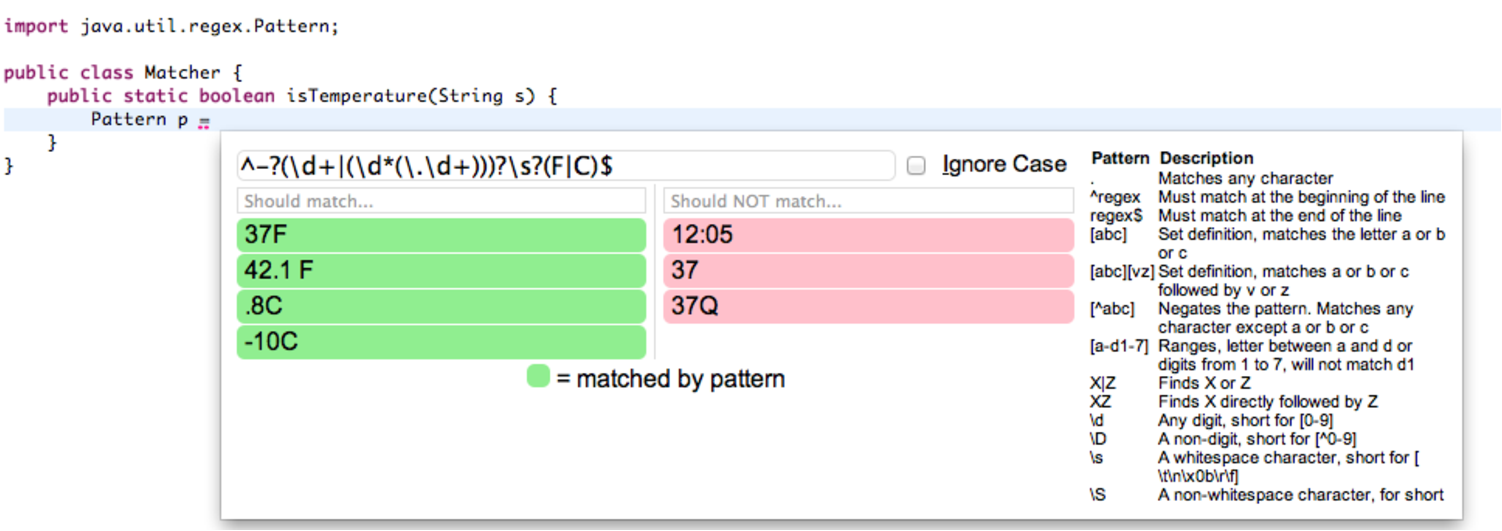
\includegraphics[scale=.55]{regex-palette.pdf}\\
% $\Downarrow$ \text{(pressing \textbf{Enter})}\\
% 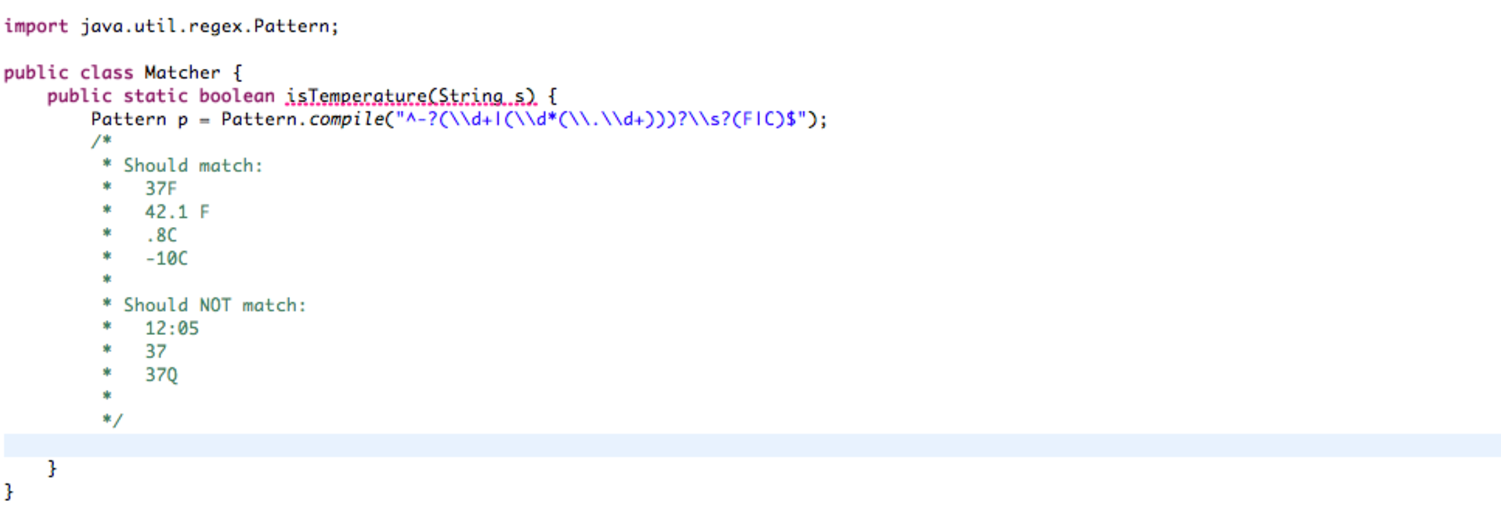
\includegraphics[scale=.55]{regex-code-generated.pdf}
% \end{center}
% \vspace{-20px}
% \caption{An example of type-specific editor services, here shown for Java.}
% \label{fig:regex-palette}
% %\vspace{-10px}
% \end{figure}

%In a conventional \emph{monolithic} programming system, support for each of these features would need to be built into the language and tools. 

To encode the concrete syntax of patterns, regular expression library providers usually provide a utility function that converts strings to patterns. Because there may be many pattern implementations, the usual approach is to define a parameterized module (a.k.a. \emph{functor} in SML) defining such utility functions generically, like this:

\begin{lstlisting}[numbers=none]
module PatternUtil(P : PATTERN)
  fun parse(s : string) : P.t
    (* ... pattern parser here ... *)
\end{lstlisting}
This allows the client of any module \lstinline{P : PATTERN} to use the following definitions:
\begin{lstlisting}[numbers=none]
module PU = PatternUtil(P)
let pattern = PU.parse
\end{lstlisting}
to construct patterns like this:
\begin{lstlisting}[numbers=none]
pattern "SSTRA|T|G|CESTR"
\end{lstlisting}
 %Again, none of our goals are comprehensively achieved.
This approach is imperfect for several reasons:
\begin{enumerate} 
\item Our first problem is syntactic (or, one might say, aesthetic): string escape sequences conflict syntactically with pattern escape sequences. For example, the following will not be well-formed:
\begin{lstlisting}[numbers=none,mathescape=|]
let ssn = pattern "SSTR\d\d\d-\d\d-\d\d\d\dESTR"
\end{lstlisting}
In fact, when compiling an analagous term using SML of New Jersey (SML/NJ), we encounter the rather puzzling error message \verb|Error: unclosed string|. Using \verb|javac|, we encounter \verb|error: illegal escape character|. In a small lab study, we observed that this error was common, and nearly always initially misinterpreted by even experienced programmers who hadn't used regular expressions recently \cite{Omar:2012:ACC:2337223.2337324}. The workaround is to  double backslashes:
\begin{lstlisting}[numbers=none]
let ssn = pattern "SSTR\\d\\d\\d-\\d\\d-\\d\\d\\d\\dESTR"
\end{lstlisting}


\item Our second problem has an impact on both correctness and performance: pattern parsing does not occur until the pattern is evaluated. For example, the following malformed pattern will only trigger an error when this term is evaluated during the full moon: %Achieving this goal is an explicit goal of this proposal, so we are obviously not happy with this.

\begin{lstlisting}[numbers=none]
case moon_phase
  Full => pattern "SSTR(GCESTR" (* malformedness not statically detected *)
  _ => (* ... *)
\end{lstlisting}
Such issues can be found via testing, but empirical data gathered from open source projects suggests that there are many malformed regular expression patterns that are not detected by a project's test suite ``in the wild'' \cite{spishak2012type}. 

Parsing patterns at run-time also incurs a performance penalty. To avoid incurring it every time the pattern is encountered during evaluation, an appropriately tuned caching strategy must be introduced, increasing client complexity.% Regular expressions are often used across large datasets in scientific applications, so the absolute peformance penalty can be non-trivial.

\item The final problem is that using strings to introduce patterns makes it more likely that programmers will use string concatenation to construct patterns derived from other patterns or from user input. For example, consider the following function:
\begin{lstlisting}[numbers=none,escapechar=|]
fun example_rx(name : string)
  pattern (name ^ "SSTR: \\d\\d\\d-\\d\\d-\\d\\d\\d\\dESTR")
\end{lstlisting}
The (unstated) intent here is to treat \lstinline{name} as a pattern matching only itself, but this is not the observed behavior when \lstinline{name} contains special characters that are meaningful in patterns. The correct code is more verbose, again resembling abstract syntax: 
\begin{lstlisting}[numbers=none]
fun example_fixed(name : string)
  P.Seq(P.Str(name), P.Seq(pattern "SSTR: ESTR", ssn)) (* ssn as above *)
\end{lstlisting}

The mistake was the result of a programmer using a flawed heuristic, so it could be avoided with sufficient developer discipline. 
The problem is that it is difficult to enforce this discipline mechanically. Both functions above have the same type and behave identically at many inputs, particularly those that would be expected during typical executions of the program (i.e. alphabetic names). In applications that query sensitive data, failures of this variety are observed to be both common and catastrophic from the perspective of security \cite{owasp2013}. Ideally, our library would be able to make it more difficult to inadvertently introduce subtle security bugs like this.
\end{enumerate}
% \begin{enumerate}
% \item \textbf{Conventional Concrete Syntax.} Patterns must be written in exactly the conventional manner, shown in blue below. Curly braces serve as an ``unquote'' form to splice one pattern into another:
% \begin{lstlisting}[numbers=none]
% let N : Pattern = /SURLA|T|G|CEURL/
% let BisI : Pattern = /SURLGC{EURLNSURL}GCEURL/
% let twoDigits : Pattern = /SURL\d\dEURL/\end{lstlisting}

% %The choice of delimiter, i.e. matching forward slashes here, is not important.
% %The cognitive load of reading and writing patterns is low and patterns are parsed once at compile-time. 
% \item \textbf{Compile-Time Parsing.} Pattern parsing must occur at compile-time, i.e. it must not incur run-time cost and malformed patterns, e.g. \lstinline{/SURLGC(EURL/}, must result in {compile-time} errors no matter where they appear in the program. 
% \item \textbf{Security By Default.} Strings must not be treated as patterns, nor used idiomatically to construct patterns. For example, the function below must be ill-typed because \lstinline{name} is not of type \lstinline{Pattern}:
% \begin{lstlisting}[numbers=none]
% fun example(name : string) : Pattern
%   let twoDigits : Pattern = /SURL\d\dEURL/
%   /SURL{EURLnameSURL}: {EURLtwoDigitsSURL}EURL/
% \end{lstlisting}
%     It is also acceptable for \lstinline{example("SSTR[a-z]ESTR")} to be equivalent to \lstinline{/SURL\[a-z\]: \d\d/}, i.e. strings are treated as patterns matching only themselves. 
% It is \emph{not} acceptable for \lstinline{example("SSTR[a-z]ESTR")} to be equivalent to \lstinline{/SURL[a-z]: \d\d/}. 

%     This is a security issue because if \lstinline{name} is derived from user input, such confusion could lead to \emph{injection attacks}, which are both common and catastrophic when using regular expression libraries that fail to achieve these goals, discussed below \cite{owasp2013}. 
%   %\item A more advanced semantics might ensure that out-of-bounds backreferences to a captured group do not occur \cite{spishak2012type}. For example, we would want \verb|BisI|, above, to have the more precise type \lstinline{Pattern(1)}, i.e. a pattern with one captured group. 
% % \end{enumerate}
% %When an error is found, an intelligible error message is provided.
% %\item An \textbf{implementation} that partially or fully compiles known regular expressions into the efficient internal representation that will be used by the regular expression matching engine (e.g., a finite automata \cite{Thompson:1968:PTR:363347.363387}) ahead of time. In most languages, this compilation step occurs at run-time, even if the pattern is fully known at compile-time, thereby introducing performance overhead into programs. If the developer is not careful to cache compiled representations, regular expressions used repeatedly in a program might be needlessly re-compiled on each use. %By performing this step ahead-of-time, these dangers can be avoided.
% %\item A range of \textbf{editor services} that support syntax highlighting for patterns, retrieval of relevant documentation, interactive testing, and pattern extraction from example strings have been shown to be helpful for programmers when working with complex regular expressions \cite{ACC_VLHCC}. An example of some of these is shown in Figure \ref{fig:regex-palette}: the editor service shown helps programmers generate correct code, here via the Java standard library's implementation of regular expressions (discussed below).
% \end{enumerate}
% Let us consider the ways that providers of regular expression libraries commonly choose to define the type \verb|Pattern|: as synonymous to \lstinline{string}, as a recursive sum type, or as an abstract type.

% \vspace{-5px}
% \paragraph{Patterns as Strings} The most na\"ive choice is to define \lstinline{Pattern} as synonymous to \lstinline{string}:

% \begin{lstlisting}[numbers=none]
% type Pattern = string
% \end{lstlisting}
% The only reason to consider this definition is that it allows us to approximate pattern syntax using standard string literal syntax:

% \begin{lstlisting}[numbers=none]
% let N : Pattern = "SSTRA|T|G|CESTR"
% \end{lstlisting}
% To splice one pattern into another, we can perform string concatenation:
% \begin{lstlisting}[numbers=none,escapechar=|]
% let BisI : Pattern = "SSTRGCESTR" ^ N ^ "SSTRGCESTR"
% \end{lstlisting}
% or use string interpolation (as in Scala or SML/NJ using quotation/antiquotation \cite{SML/Quote}):
% \begin{lstlisting}[numbers=none,mathescape=|]
% let BisI : Pattern = s"SSTRGC${ESTRNSSTR}GCESTR"
% \end{lstlisting}

% Though this comes close, goal 1 is not truly achieved because the syntax of strings can conflict with the syntax for patterns. 

% Goal 2 is not achieved because parsing occurs only at run-time when we match a string against a pattern (worse, every time we do so unless the implementation uses an effective caching strategy).

% Goal 3 is also not achieved because the following code typechecks:
% \begin{lstlisting}[numbers=none,mathescape=|]
% fun example_bad_1(name : string) : Pattern
%   let twoDigits : Pattern = "SSTR\\d\\dESTR"
%   s"SSTR${ESTRnameSSTR}-${ESTRtwoDigitsSSTR}"ESTR
% \end{lstlisting}
% but \lstinline{example_bad_1("SSTR[a-z]ESTR")} evaluates to \lstinline{"SSTR[a-z]-\\d\\dESTR"}.



% \paragraph{Patterns as Recursive Sums} A more semantically justifiable strategy is to define \lstinline{Pattern} as a recursive sum type  \cite{pfpl}. Wyvern supports these in the form of case types, which are analagous to datatypes in ML:

% \begin{lstlisting}[numbers=none]
% casetype Pattern
%   Empty
%   Str of string
%   Seq of Pattern * Pattern
%   Or of Pattern * Pattern
%   Star of Pattern  
% \end{lstlisting}

% More generally, we can hold the representation of patterns abstract while exposing an isomorphic interface to clients by defining an abstract type in a {module} opaquely ascribed the following {module type} (a.k.a. \emph{signature} in SML): % exposes the constructors and case analysis as functions:

% \begin{lstlisting}[deletekeywords={case},numbers=none]
% module type PATTERN
%   type t
%   val Empty : t
%   val Str : string -> t
%   val Seq : t * t -> t
%   val Or : t * t -> t
%   val Star : t -> t
%   val case : (
%     'a -> 
%     (string -> 'a) ->
%     (t * t -> 'a) ->
%     (t * t -> 'a) ->
%     (t -> 'a) ->
%     'a)
% \end{lstlisting}
% The client of any module \lstinline{P : PATTERN} can define \verb|Pattern| as synonymous to \verb|P.t|: 
% \begin{lstlisting}[numbers=none]
% type Pattern = P.t
% \end{lstlisting}



%The first one might not be found incorrect without rigorous testing with unexpected inputs. Goal 3 expresses the ideal of designing a language where security does not require considering such subtle issues extralinguistically.%This is precisely why injection attacks are so difficult to detect.

% The dialect of Standard ML implemented by SML/NJ, recognizing that directly using constructors is often less than ideal, provides a facility for quotation/antiquotation \cite{SML/Quote}, which if introduced into Wyvern could be used as follows:
% \begin{lstlisting}[numbers=none,escapechar=|,mathescape=|]
% fun example(p : string)
%   let twoDigits = P.qparse `SQT\d\dEQT`
%   P.qparse `SQT^(EQTP.Str(p)SQT)-^(EQTtwoDigitsSQT)EQT`
% \end{lstlisting}

% Here, backticks are used to indicate a quoted term within which carets serve as an antiquote operator. This still represents a  compromise against goal 1. The most serious problem is that, once again, parsing does not occur until run-time. There are also  conflicts between quotation syntax and pattern syntax, i.e. \verb|^| conventionally means character set negation inside patterns, which conflicts with antiquotation here. This mechanism also does not support antiquotation at more than one type, so we could not define the antiquote operator to insert the \verb|Str| constructor automatically, as suggested in goal 3. %For syntax that necessary involves antiquotation at multiple types (e.g. concrete syntax for a programming language with multiple syntactic sorts, HTML which might include Javascript and CSS, and others), this 

\subsection{Existing Approaches}\label{sec:syntax-existing} These problems with string-oriented approaches to concrete syntax arise in many similar scenarios \cite{TSLs}, motivating  research on more direct syntax extension mechanisms \cite{Bravenboer:2007:PIA:1289971.1289975}.

The simplest such mechanisms are those where each new syntactic form is described by a single equation. For example, the surface language of Coq (called Gallina) includes such a mechanism \cite{Coq:manual}. A theoretical account of such mechanisms has been developed by Griffin \cite{5134}. Unfortunately, these mechanisms are not able to express pattern syntax in the conventional manner for various reasons. For example, sequences of characters should not be parsed as identifiers.


Syntax extension mechanisms based on context-free grammars like  Sugar* \cite{erdweg2013framework}, Camlp4 \cite{ocaml-manual} and many others are more expressive, and would allow us to directly introduce pattern syntax into our base language's grammar. However, this is perilous because none of the mechanisms described thusfar guarantee \emph{syntactic composability}, i.e. as stated in the Coq manual, ``mixing different symbolic notations in [the] same text may cause serious parsing ambiguity''. If another library provider used similar syntax for a different variant of regular expressions, or for an entirely unrelated abstraction, then a client could not simultaneously use both libraries in the same scope. % Resolving such parsing amibiguities is left to each client of the library. 

In response to this problem, Schwerdfeger and Van Wyk have developed a modular analysis that accepts only syntax extensions that use a unique starting token and satisfy some subtle conditions on follow sets of base language non-terminals \cite{conf/pldi/SchwerdfegerW09}. However, simple starting tokens like \lstinline{pattern} cannot be guaranteed to be globally unique, so we would need to use a more verbose token like \lstinline{edu_cmu_wyvern_rx_pattern}. There is no simple, principled way to define scoped abbreviations for starting tokens because this mechanism is language-external.

In any case, we must now decide how our newly introduced derived forms desugar to forms in our base language, which in this case requires determining which module the constructors the desugaring uses will come from. Clearly, simply assuming that a module named \lstinline{P} satisying \lstinline{PATTERN} is in scope is a brittle solution. Indeed, we should expect that the extension mechanism actively prevents such capture of specific variable names to ensure that variables (including module variables) can be freely renamed. However, we note that such \emph{hygiene mechanisms} are only well-understood when performing term-to-term rewriting (as in Lisp-style \emph{macro systems}\todo{citation}) or simple equational systems like those found in Coq. For more flexible mechanisms, the issue is a topic of ongoing research (none of the grammar-based mechanisms described above enforce hygiene).

Putting aside the question of hygiene, we can address the problem by requiring that the client explicitly identify the module the desugaring should use:
\begin{lstlisting}[numbers=none]
let N = edu_cmu_wyvern_rx_pattern[P] /A|T|G|C/
\end{lstlisting}
Syntactically, this is the best we can do using existing approaches.  

These approaches further suffer from a paucity of direct reasoning principles, i.e. the program can only be reasoned about post-desugaring. Given an unfamiliar piece of syntax, there is no simple method for determining what type it will have, or even for identifying which extension determines its desugaring, causing difficulties for both humans (related to code comprehension) and tools. 

% \begin{enumerate}
% \item Given an unfamiliar piece of syntax, there is no simple method for determining what type it has, or to identify which extension determines its desugaring, hindering code comprehension.
% \item It requires that the syntax be expressed as a grammar that can be consumed by a particular parser generator. Not all syntax  is most naturally expressed in this way, but there is no way to use a ``hand-rolled'' parser.
% \end{enumerate}

\subsection{Contributions}\label{sec:syntax-contributions}
We propose designing a  syntax extension mechanism that addresses all of the problems just described. It consists of two constituent concepts:
\begin{itemize}
\item The concept that the mechanism is oriented around is the \emph{typed syntax macro} (TSM). %A TSM is applied to a \emph{delimited form}, which can contain  arbitrary syntax in its \emph{body}, and zero or more module or type parameters. Based on the body of the delimited form, the TSM statically computes an elaboration to a {base form}. 
For example, consider the following concrete term:
\begin{lstlisting}[numbers=none]
pattern[P] /SURLA|T|G|CEURL/
\end{lstlisting}

The TSM \lstinline{pattern} is being applied to a module parameter, \lstinline{P}, and a \emph{delimited form}, \lstinline{/SURLA|T|G|CEURL/}. This term elaborates \emph{statically} to the following:

% import cs.cmu.edu/~wyvern/regex as R
% let syntax pattern = R.pattern
% let module P = R.P
% The first line imports our top-level regular expression module (identified uniquely by a URI) and binds a shorter name, \lstinline{R}, to it. The second line binds a local name to the  TSM named \lstinline{pattern} that \lstinline{R} exports. The third line gives a shorter name, \lstinline{P}, to the module \lstinline{R.P : R.PATTERN}, as defined previously. The fourth line then applies \lstinline{pattern} to this module parameter and a form delimited by forward slashes. This causes it to elaborate \emph{statically} to the following base form:
\begin{lstlisting}[numbers=none]
P.Or(P.Str "SSTRAESTR", P.Or(P.Str "SSTRTESTR", P.Or(P.Str "SSTRGESTR", P.Str "SSTRCESTR")))
\end{lstlisting}

The TSM is defined as shown below:
\begin{lstlisting}[numbers=none]
syntax pattern[P : PATTERN] for P.t
  fn (ps : ParseStream) => (* pattern parser here *)
\end{lstlisting}
We declare a module parameter (calling it \lstinline{P} here is unimportant, i.e. the TSM can be used with \emph{any} module satisfying module type \lstinline{PATTERN}), and the type clause \lstinline{for P.t}, which guarantees that any use of this TSM will either be ill-typed or elaborate to a term of type \lstinline{P.t}. The elaboration is computed by the compile-time action of the parse function defined in the indented block above. This function must be of type \lstinline{ParseStream -> Exp}, where the type \lstinline{ParseStream} gives the function access to the \emph{body} of the delimited form (in blue above) and the type \lstinline{Exp}  encodes the abstract syntax of the base language. Both types are defined in the Wyvern prelude, which is a set of definitions available ambiently.

When the type of the term is known, e.g. due to a type annotation on the let binding, the module parameter \lstinline{P} can be inferred:
\begin{lstlisting}[numbers=none]
let N : P.t = pattern /SURLA|T|G|CEURL/
\end{lstlisting}

TSMs can be abbreviated using a let-binding style mechanism:
\begin{lstlisting}[numbers=none]
let syntax pat = pattern[P]
pat /SURLA|T|G|CEURL/
\end{lstlisting}

TSMs can parse portions of the body of the delimited form as a base language term, to support splicing syntax:
\begin{lstlisting}[numbers=none]
let N = pat /SURLA|T|G|CEURL/
let BisI = pat /SURLGC({EURLNSURL})GCEURL/
\end{lstlisting}
A hygiene mechanism ensures that only those portions of the elaboration derived from such spliced terms can refer to variables in the surrounding scope.

Strings are never involved, so the attendant security issues described previously are easily avoidable. That is, the following 

\item To support an even more concise usage profile, Wyvern also  supports \emph{type-specific languages} (TSLs), which allow library providers to associate a TSM directly with a declared type. For example, the module \lstinline{P} above can associate \lstinline{pattern} with \lstinline{P.t}. Local type inference then determines which TSM is applied implicitly to handle a form not prefixed by a TSM name. For example, the following is equivalent to the above:
\begin{lstlisting}[numbers=none]
let N : P.t = /SURLA|T|G|CEURL/
\end{lstlisting}
\end{itemize}
\subsubsection{Typed Syntax Macros (TSMs)}\label{sec:tsms}
For simplicitly, let us begin with a typed syntax macro providing pattern syntax using the case type encoding above:
\begin{lstlisting}[numbers=none]
syntax pattern => Pattern = e_parser
\end{lstlisting}
The term \lstinline{e_parser}, elided here, must have type \lstinline{ParseStream -> Exp}, where \lstinline{ParseStream} classifies a sequence of characters and \lstinline{Exp} classifies a reified Wyvern expression. 

\subsubsection{Type-Specific Languages (TSLs)}\label{sec:tsls}

\subsection{Timeline}\label{sec:syntax-timeline}
SAC, ECOOP.

TODO: module-parameterized TSMs

\section{Extensible Semantics}\label{sec:extensible-semantics}


\subsubsection{Example 2: Regular Strings}\label{sec:rstr}
The example above deals with how regular expression patterns are  encoded, introduced and reasoned about. Going further, programmers may also benefit from a semantics where they can statically constrain strings to be within a particular regular language \cite{sanitation-psp14}. For example, a programmer might want to ensure that the arguments to a function that creates a database connection given a username and password are alphanumeric strings, ideally including this specification directly in the type of the  function:
\begin{lstlisting}[numbers=none]
type alphanumeric = rstring /SURL[A-Za-z0-9]+EURL/
val connect : (alphanumeric * alphanumeric) -> DBConnection
\end{lstlisting}

This example requires that the language include a {type constructor}, \verb|rstring|, indexed by a statically known regular expression, written using the syntax described above. Ideally, we would be able to use standard string literal syntax for such regular strings as well, e.g.
\begin{lstlisting}[numbers=none]
let connection = connect("admin", "password")
\end{lstlisting}

To be useful, the language would also need a static semantics for standard operations on regular strings. For example, concatenating two alphanumeric strings  should result in an  alphanumeric string. This should not introduce additional run-time cost as compared to the corresponding operations on standard strings. Coercions that can be determined statically to be valid in all cases due to a language inclusion relationship should have trivial cost, e.g. coercions from alphabetic to alphanumeric strings.

Regular strings might go beyond simply \emph{refining} standard string types (i.e. specifying verification conditions atop an existing semantics \cite{Freeman91}). For example, they might define an operation like \emph{captured group projection} that has no analog over standard strings:
\begin{lstlisting}[numbers=none]
let example : rstring /SURL(\d\d\d)-(\d\d\d\d)EURL/ = "555-5555"
let group0 (* : rstring /\d\d\d/ *) = example#0
\end{lstlisting}
It should be possible to give this operation a cost of $\mathcal{O}(1)$. %From a language implementation perspective, this requires that different regular string types  have different representations, also not possible when using a refinement system over strings. %This is not possible if regular strings are defined using a refinement system atop a language with only strings. %This example requires introducing new operators into the system that did not already exist, and using an underlying represention that differs for different type indices. 

\subsubsection{Example 3: Labeled Products with Functional Update Operators}\label{sec:lprod}
The simplest way to specify the semantics of product types is to specify only nullary and binary products \cite{pfpl}. However, in practice, many more general but also more complex variations on product types are built in to various dialects of ML and other languages, e.g. $n$-ary tuples, labeled tuples, 
records (identified up to reordering), 
records with width and depth coercions \cite{Cardelli:1984:SMI:1096.1098} and records with functional update operators (also called \emph{extensible records}) \cite{ocaml-manual}. {The Haskell wiki notes that ''extensible records  are not implemented in GHC. The problem is that the record design space is large, and seems to lack local optima. [...] As a result, nothing much happens.'' \cite{GHCFAQ}}%, 
 %mutable fields \cite{ocaml-manual}, 
%field delegation \cite{atlang-gpce14} \todo{gpce submission} 
%and 
% ``methods'' (i.e. pure objects) \cite{TSLs}


We would ideally like to avoid needing the language designer to decide \emph{a priori} on just one privileged point in this large design space. Instead, the language designer might define only nullary and binary products, and include an extension mechanism that makes it possible for these other variations on products to be defined as libraries and  used together without conflict. For example, we would like to define the semantics of labeled products, which have labeled rows like records but maintain a row ordering like tuples, in a library. An example of a labeled product type (constructed by the type constructor \lstinline{lprod}) classifying conference papers might be:
\begin{lstlisting}[numbers=none]
type Paper = lprod {
  title : rstring /SURL.+EURL/,
   conf : rstring /SURL[A-Z]+ \d\d\d\dEURL/
}
\end{lstlisting}

The row ordering should make it possible to introduce values of this type either with or without explicit labels, e.g.
\begin{lstlisting}[numbers=none]
fun make_paper(t : rstring /SURL.+EURL/) : Paper = {title=t, conf="EXMPL 2015"}
\end{lstlisting}
should be equivalent to
\begin{lstlisting}[numbers=none]
fun make_paper(t : rstring /SURL.+EURL/) : Paper = (t, "EXMPL 2015")
\end{lstlisting}
(note that we aim to be able to unambiguously re-use standard record and tuple syntax.)

We should then be able to project out rows by providing a positional index or a label:
\begin{lstlisting}[numbers=none]
let test_paper = make_paper "Test Paper"
test_paper#0
test_paper#conf
\end{lstlisting}

We might also want our labeled tuples to support functional update operators. For example, an operator that dropped a row might be used like this:
\begin{lstlisting}[numbers=none]
let title_only (* : lprod {title : rstring /.+/} *) = test_paper.drop[conf]
\end{lstlisting}
An operation that added a row, or updated an existing row, might be used like this:
\begin{lstlisting}[numbers=none]
fun with_author(p : Paper, a : rstring /SURL.+EURL/) = p.ext(author=a)
\end{lstlisting}
% \subsection{Language-External Approaches}\label{external-approaches}


% In situations like these where a library-based approach is not satisfactory, providers must today take a \emph{language-external approach}, specifying a new system dialect, reasoning about its metatheory monolithically and implementing it using a {compiler generator} \cite{brooker1963compiler}, {language workbench} \cite{erdweg2013state}, {DSL framework} \cite{fowler2010domain}, an extension mechanism for a {particular} compiler\footnote{Compilers that modify, or allow modification of, the semantics of their base language, rather than simply permitting semantics-preserving optimizations, should be considered a pernicious means for creating dialects. 
% %That is, some programs that purport to be written in C, Haskell or Standard ML are actually written in compiler-specific dialects of these languages.
% }, editor or other tool, or by forking an existing system implementation. 

% For example, a researcher interested in providing the regular expression related features just described (let us refer to these collectively as \texttt{R}) might design a new system with built-in support for them, perhaps basing it on an existing system containing standard general-purpose features, \texttt{G} (e.g. the features of Standard ML). A different researcher developing a new language-integrated parallel programming abstraction, \texttt{P}, might  take the same approach (e.g. Manticore is such a system based on SML \cite{conf/popl/FluetRRSX07}). A third researcher, developing a type system for reasoning about units of measure (\texttt{Q}) might again do the same \cite{conf/cefp/Kennedy09}. This results in a collection of  systems, as diagrammed in Figure \ref{approaches}a. 

% Although these systems are valid ``proofs of concept'', this is a rather weak notion because no abstraction will be used entirely in isolation. Such an approach gives us no rigorously justifiable  reason to believe that it can safely and naturally be merged with others specified or implemented in the same way. That is, one must either use the system defining features \texttt{G+R}, \texttt{G+P} or \texttt{G+Q}. There is no system defining \texttt{G}, \texttt{R}, \texttt{P} and \texttt{Q} in other combinations. % and there is no formal, general mechanism for merging these systems.
% We argue that, due to these problems of composition, taking a language-external approach to realizing a new feature should be considered harmful and avoided whenever possible. 

% \begin{figure}
% \begin{center}
% 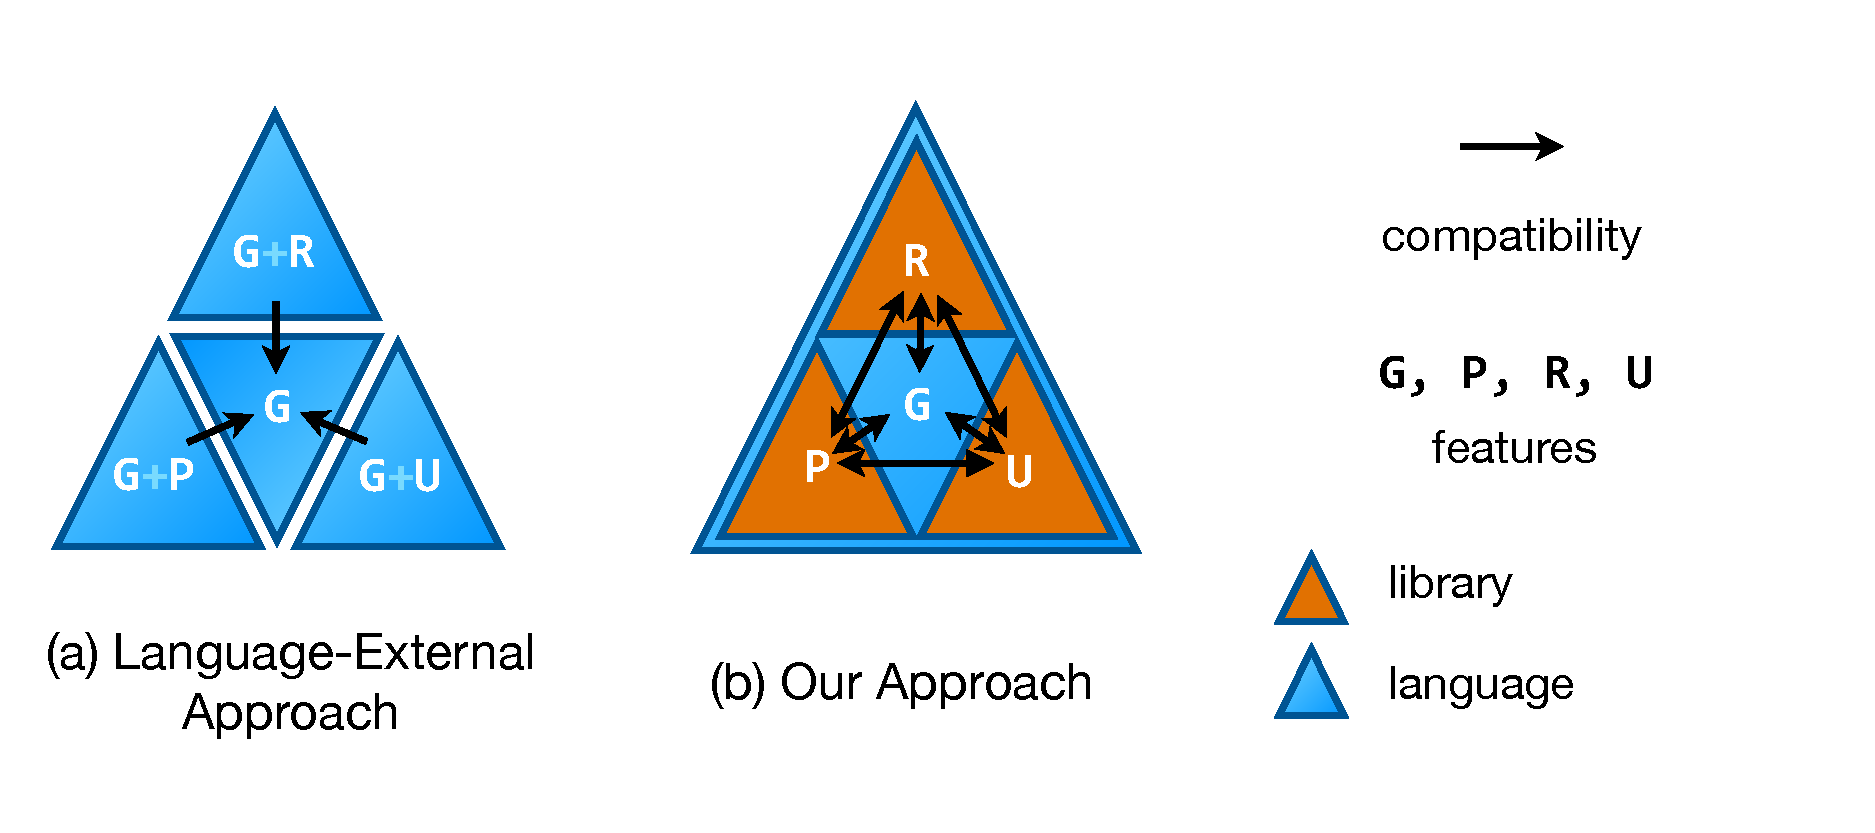
\includegraphics[scale=.48]{approaches.pdf}
% \end{center}
% \vspace{-20px}
% \caption{\small (a) When taking a language-external approach, new features are packaged together into separate languages and tools. (b) We propose an approach where there is one extensible host language and the compile-time and edit-time logic governing new constructs is expressed within safely composable libraries.}
% \label{approaches}
% %\vspace{-10px}
% \end{figure}
%  %
% % More specifically, there is no guarantee of \textbf{orthogonality} or even \textbf{interoperability}.% This has limited the broad adoption of these kinds of innovations.%This latter method couples the semantics of the feature to the implementation details of a particular tool. Because the use of one implementation entails a different semantics for the feature than another, the extended tool acts, \emph{de facto}, as a distinct system for our purposes. 

% %\paragraph{Orthogonality} Features implemented by language-external means like these cannot be adopted individually, but instead are only available coupled to a fixed collection of other features. This makes adoption more costly when these incidental features are  not desirable or are insufficiently developed (``toy languages''), or when the features bundled with a different language or tool are simultaneously desirable. 

% % Recent evidence indicates that this is one of the major barriers preventing research  from being driven into practice. For example, developers prefer high-level language-integrated parallel programming abstractions that provide  stronger semantic guarantees  \cite{cave2010comparing}, but library-based approximations are far more widely adopted because the ``parallel programming languages'' privilege only a few  specialized abstractions at the language level. In contrast, it is widely acknowledged that  different specialized abstractions are more appropriate in different situations \cite{Tasharofi:2013rc}. Moreover,  parallel programming is rarely the only relevant specialized concern. Support for regular expressions as above would be simultaneously desirable for processing large amounts of genomic data in parallel.% but using these features together in the same compilation unit would be difficult or impossible if implemented using language-external means. Indeed, switching to a ``parallel programming language'' would likely make it \emph{more} difficult to use regular expressions, as these are likely to be less well-developed in a specialized language than in an established general-purpose language.% This intuition was perhaps most succinctly expressed by a participant in a recent study by Basili et al. \cite{basili2008understanding}:  ``I hate MPI, I hate C++. [But] if I had to choose again, I would probably choose the same.'' %Similarly, a language and tools designed primarily to support regular expressions might make an interesting research project, but it would not be a suitable tool for writing large applications with more varied needs.

% %\item Developing a new language and its associated tools places a significant development burden on providers who may wish only to promote a few core innovations, although tools like compiler generators, language workbenches and easy-to-extend tools can decrease this burden. 
% %\item 

% %Clients seem to prioritize the ability to choose different features for different portions of an application. 
% %If calling between languages were safe and easy, then using a variety of specialized languages and associated tools might be less problematic. In fact, s
% %Recognizing the limitations of relying on monolithic collection of primitives, some researchers have advocated instead for a model where multiple languages used within a single application, calling it the \emph{language-oriented approach} to software development \cite{languageoriented}. 

% % \paragraph{Interoperability} Even in cases where, for each component of a software system, a programming system considered entirely satisfactory by its developers is available (e.g. a team goes through the trouble of implementing \verb|G+R+P| by reading papers about \verb|G+R| and \verb|G+P| and disentangling orthogonality-related issues), there remains a problem at any interface between  components written using a different combination of features. An interface that  externally exposes a specialized construct particular to one language (e.g. a function that requires a quantity having a particular unit of measure) cannot necessarily be safely and naturally consumed from another language (e.g. a parallel programming language). Tool support is also lost when calling into different languages. %We call this the \emph{interoperability problem}. % programs written by clients of a certain collection of features cannot always interface with programs written by clients of other features  in a safe, performant and natural manner.

% % One strategy taken by proponents of a {language-oriented approach} \cite{journals/stp/Ward94} to partially address the interoperability problem is to  target an established intermediate language and use its constructs as a common language for communication between components written in different languages. Scala \cite{200464/IC} and F\# \cite{pickering2007foundations} are examples of prominent general-purpose languages that have taken this approach, and most DSL frameworks also rely on this strategy. As indicated in Figure \ref{approaches}a, this only enables interoperability in one direction. Calling into the common language becomes straightforward and safe, but calling in the other direction, or between the languages sharing the common target, does not, unless these languages are only trivially different from the common language. 

% % %This approach only works well when new languages consist of constructs that can also be expressed safely and almost as naturally in the common language.
% % %But many of the most innovative constructs found in modern languages (often, those that justify their creation) are difficult to define in terms of existing constructs in ways that guarantee all necessary invariants are statically maintained and that do not require large amounts boilerplate code and run-time overhead. 
% % As a simple example with significant contemporary implications, F\#'s type system does not admit \verb|null| as a value for any type both defined and used within F\# code, but maintaining this sensible internal invariant still requires dynamic  checks because the stricter typing rules of F\# do not apply when F\# data structures are constructed by other languages on the Common Language Infrastructure (CLI) like C\# or SML.NET. This is not an issue exclusive to intermediate languages that make regrettable choices regarding \verb|null|, however. The F\# type system also includes support for checking that units of measure are used correctly \cite{syme2012expert, kennedy1994dimension}, but this more specialized static invariant is left entirely unchecked at language boundaries. Indeed, guidelines for F\# suggest that exposing functions that operate over values having units of measure, datatypes or tuples is not recommended when a component ``might be used'' from another language \cite{syme2012expert} because it is awkward to construct and consume these from other languages without the convenient primitive operations (e.g. pattern matching) and syntax that F\# includes. SML.NET prohibits exposing such types at component boundaries altogether. Moreover, it also cannot naturally consume F\# data structures, despite having a rather similar syntax and semantics in most ways (both languages directly descend from ML). 
% %In Scala, traits that have default method implementations are difficult to implement from Java or other JVM languages and the workaround can break if the trait is modified \cite{scalatraitinterop}. 
% %In some cases, desirable features must be omitted entirely due to concerns about interoperability. F\#, for example, aimed to retain source compatibility with Ocaml code, but due to the need for bidirectional interoperability with CLI languages, it does not support features like polymorphic variants, modules or functors \cite{ocaml-manual} because they have no apparent analogs in the type system of the CLI.
% %\end{itemize}

% %\subsection{Language-Integrated Approaches}\label{language-integrated-approaches}


% %Such libraries have been called \emph{active libraries}  \cite{activelibraries}. %Features implemented within active libraries can be imported individually, unlike features implemented by external means, giving us a potential means to avoid the problems of orthogonality and interoperability just described.

% % We must proceed with caution, however: critical issues having to do with {safety} must be overcome before language-integrated extension mechanisms can be introduced into a system. If too much control over  these core features of the system is given  to developers, the system's metatheory may become weak. 
% % %For example, an extension could weaken important metatheoretic guarantees previously provided by the system. 
% % For example, parsing ambiguities might arise if the syntax can be modified arbitrarily. Type safety  may not hold if the static and dynamic semantics of the language can be modified or extended arbitrarily from within libraries. Furthermore, even if extensions can be shown not to cause such problems in isolation, there may still be conflicts between extensions that could weaken their semantics, leading to subtle problems that only appear when two extensions are used together. %As a simple example, if two active libraries introduce the same syntactic form but back it with differing (but individually valid) semantics, this ambiguity  would only manifest itself when both libraries were imported within the same scope. %Resolving these kinds of ambiguities requires significantly more expertise with parser technology than using the syntax itself does. 
% % These issues have plagued previous attempts to design language-integrated extensibility mechanisms.\todo{I can include a more detailed related work section if requested.}% We will briefly review some of these attempts below, then return to our approach.% To prevent them, our mechanisms will organize  extension logic around types to guarantee that extensions are both safe in isolation and also safely composable in any combination. 


%  %This represents a minimalist approach to system design -- the conventional distinction between built-in and user-defined constructs is blurred and most features of the system are orthogonally implemented as {libraries}, rather than by the maintainers of the system.

% %The mechanisms we describe will do so primarily by delimiting the scope of an extension to expressions of a single user-defined type or family of types. 

% %This can be thought of as a more pernicious form of the conflict that arises when two globally-accessible constructs are given the same name. n languages without universal namespacing mechanisms (e.g. C, JavaScript, \LaTeX, ML and many others). 

% %The extension mechanism\todo{elaborate on safety requirements + tension between expressiveness and safety, merge with next paragraph}. must be expressive enough to allow users to associate rich run-time, compile-time and edit-time behaviors with user constructs directly, while being sufficiently restrictive to maintain the global safety properties of the language and system as a whole, and to ensure that constructs cannot interfere with one another. 
